\section{Theorie}

\subsection{Spinbewegung im Magnetfeld}

Wird ein Atomkern mit einem Kernspin $I>0$ betrachtet, so besitzt dieser ein magnetisches Moment
\begin{equation*}
  \vec{\mu} = \gamma \vec{I}
\end{equation*}
mit dem gyromagnetischen Verhältnis $\gamma$.
Für Protonen mit Spin $I = \sfrac{1}{2}$ gilt
\begin{equation*}
  \gamma = 2 \pi \cdot \SI{42.577}{\mega\hertz\per\tesla}\,. %\cite{https://docs.scipy.org/doc/scipy/reference/constants.html}
\end{equation*}

In einem Magnetfeld $\vec{B_0} = B_0 \vec{e_z}$ erfährt ein Proton wegen seines magnetischen Moments ein Drehmoment $\vec{T}$.
Vereinfacht kann dieser Spin als Kreisel in dem Magnetfeld betrachtet werden.
Aus
\begin{align*}
  \vec{T} &= \vec{\mu} \times \vec{B_0}  \\
  \vec{T} &= \frac{\symup{d}\vec{I}}{\symup{d}t}
\end{align*}
folgt eine Spinpräzission
\begin{equation}
  \vec{I} =
  \begin{pmatrix*}[c]
    I_{\text{x$_0$}} \, \cos(\gamma B_0 t + \phi_0) \\
    -I_{\text{y$_0$}} \, \sin(\gamma B_0 t + \phi_0) \\
    I_{\text{z$_0$}}
\end{pmatrix*}
 \, .
\end{equation}

Der Spin des Protons präzidiert also um die Richtungsachse des B-Felds während die Anfangsphase $\phi_0$ dabei einer Gleichverteilung folgt.
Die Frequenz $\omega_0 = \gamma B_0$ wird auch als Lamorfrequenz bezeichnet.
Die Bewegung des Spins und somit auch des magnetischen Moments des Protons in x-y Richtung kann in einer Leiterschleife eine Spannung mit der Lamorfrequenz induzieren.
Für ein Volumen mit vielen Protonen wird aufgrund der Anfangsphasen jedoch keine Spannung gemessen.


Für die Komponente des Spins entlang des B$_{0}$-Feld folgt für Spin-$\sfrac{1}{2}$ Teilchen
\begin{equation*}
  I_\text{z} = \hbar m \quad \text{mit} \quad m = \pm\frac{1}{2} \, .
\end{equation*}
Die Ausrichtung der Spins entlang des Magnetfelds ist also entweder parallel (up) oder antiparallel (down) und
folgt der Boltzmann Verteilung
\begin{equation*}
  \frac{N_\text{up}}{N_\text{down}} = e^{\sfrac{\Delta E}{k_\text{B} T}} > 1
\end{equation*}
für
\begin{equation*}
  E = - \vec{\mu} \cdot \vec{B_0} = \mp \frac{1}{2} \hbar \omega_0 \Rightarrow \Delta E = \hbar \omega_0 \, .
\end{equation*}

Es sind also immer mehr Spins in dem energetisch günstigeren Zustand up und es entsteht eine feste Magnetisierung entlang des externen Magnetfelds B$_0$ (Längsmagnetisierung).

%%%%%%%%%%%%%%%%%%%%%%%%%%%%%%%%    Theorie Quermagnetisierung    %%%%%%%%%%%%%%%%%%%%%%%%%%%%%%%%%%%%%%%%

\subsection{Quermagnetisierung}

Um nun in einer Spule eine Spannung zu induzieren, wird die Langsmagnetisierung der Probe auf die x-y-Ebene gekippt und die sogenannte Quermagnetisierung erzeugt.
Dazu muss zuerst ein Koordinatensystem eingeführt werden, welches mit der Lamorfrequenz rotiert, in dem Koordinatensystem steht der Vektor des magnetischen Moments still.

Um das magnetische Moment nun auf die x-y-Ebene zu kippen, wird ein transversales Magnetfeld B$_1$ senkrecht zum ersten Magnetfeld B$_0$ eingeschaltet. Dieses, im rotierenden Koordinatensystem stehende, Magnetfeld entspricht einer linear polarisierten elektromagnetischen Welle mit der Lamorfrequenz im nicht rotierenden Koordinatensystem.
Für das Transversalfeld ergibt sich der Flipwinkel
\begin{equation*}
  \alpha = \gamma B_1 \Delta t
\end{equation*}
welcher dem Winkel entspricht, um den die Längsmagnetisierung aus der z-Achse gekippt wird, dabei bezeichnet $B_1$ die Magnetfeldstärke des Transversalfelds und $\Delta t$ die Zeit, die das Transversalfeld eingeschaltet ist.

Nach dem Puls rotiert der Vektor des magnetischen Moments in der x-y-Ebende weiter um die z-Achse.
Dies induziert in einer Spule eine Spannung mit der Lamorfrequenz, in typischen NMR Versuchen wird dazu die Spule genutzt, mit der auch das B$_1$-Feld geschaltet wird.

%%%%%%%%%%%%%%%%%%%%%%%%%%%%%%%%    Relaxation    %%%%%%%%%%%%%%%%%%%%%%%%%%%%%%%%%%%%%%%%

\subsection{Relaxation}
Durch Wechselwirkungsprozesse bleibt die Magnetisierung nicht in der x-y-Ebene, sondern relaxiert wieder in ihre Ursprungsausrichtung entlang der z-Achse.
Dies erzeugt in der Spule ein exponentiell abfallendes Spannungssignal, welches Free Induction Decay (FID) genannt wird.

%%%%%%%%%%%%%%%%%%%%%%%%%%%%%%%%    Theorie T1    %%%%%%%%%%%%%%%%%%%%%%%%%%%%%%%%%%%%%%%%

\subsubsection{Spin-Gitter Wechselwirkung: $T_1$ Zeit}

Durch Wechselwirkung der Protonen mit umliegenden Molekülen können jene, durch Abgabe von Energiequanten $\Delta E = \hbar \omega_0$, in den Grundzustand zurückfallen.
Dies ist ein statistischer Prozess, der stark von dem untersuchten Material abhängt.
Die Gesamtmagnetisierung in z-Richtung baut sich mit der Zeitkonstanten $T_1$ mit
\begin{equation}
  M_\text{z} = M_\text{z$_0$} \, (1-e^{-\sfrac{t}{T_1}})
  \label{eqn:T1Zeit}
\end{equation}
auf. Dabei beschreibt $M_\text{z$_0$}$ die Gesamtmagnetisierung vor dem Schalten des B$_1$-Feldes.

%%%%%%%%%%%%%%%%%%%%%%%%%%%%%%%%   Theorie T2    %%%%%%%%%%%%%%%%%%%%%%%%%%%%%%%%%%%%%%%%

\subsubsection{Spin-Spin Wechselwirkung: $T_2$-Zeit}

Das magnetische Feld wird durch die Anwesenheit von anderen Spins lokal gestört und es herrscht eine andere Lamorfrequenz.
Dadurch dephasieren die Spins und die Quermagnetisierung nimmt mit
\begin{equation}
  M_\text{x,y} = M_\text{x$_0$,y$_0$} \cdot e^{-\sfrac{t}{T_2}}
  \label{eqn:T2Zeit}
\end{equation}
ab.
Wegen kleiner Feldinhomogenitäten innerhalb der Messspule dephasiert das Signal nochmals schneller mit der $T_2^*$ Zeitkonstanten.
Es gilt immer $T_2^*<T_2<T_1$.
Durch die Bestimmung der Zeitkonstanten $T_1$ und $T_2$ können so Informationen über die Zusammensetzung des untersuchten Materials gewonnen werden.

%%%%%%%%%%%%%%%%%%%%%%%%%%%%%%%%   Messsequenzen    %%%%%%%%%%%%%%%%%%%%%%%%%%%%%%%%%%%%%%%%

\subsection{Messsequenzen}

Um die $T_1$- oder $T_2$-Zeit zu bestimmen werden verschiedene Pulssequenzen des B1-Pulses geschaltet.
Die $T_1$-Zeit wird in diesem Versuch durch die \textbf{Inversion-Recovery} bestimmt.
Dabei wird zu Beginn ein \SI{180}{\degree}-Puls geschaltet und die Magnetisierung auf die negative z-Achse gekippt.
Nach einer Zeit $\tau$ kippt ein \SI{90}{\degree}-Puls die Magnetisierung auf die x-y-Ebene, die Stärke der Quermagnetisierung ist dann abhängig von der Relaxation der Magnetisierung in z-Richtung mit $T_1$.

Zur Messung der $T_2$-Zeit wird in diesem Versuch die \textbf{Meiboom-Gill-Methode} genutzt.
Dabei wird zu Beginn ein \SI{90}{\degree}-Puls geschaltet um die Magnetisierung in die x-y-Ebende zu kippen.
Das Signal dephasiert daraufhin schnell mit der $T_2^*$-Zeit.
Um eine Messung des Signals zu realisieren, wird auf den Effekt des \textbf{Spin-Echo} zurückgegriffen.
Eine schematische Abbildung der Spinbewegung beim Spin-Echo ist in Abbildung \ref{fig:Spin-Echo} gezeigt.

\begin{figure}[H]
  \centering
  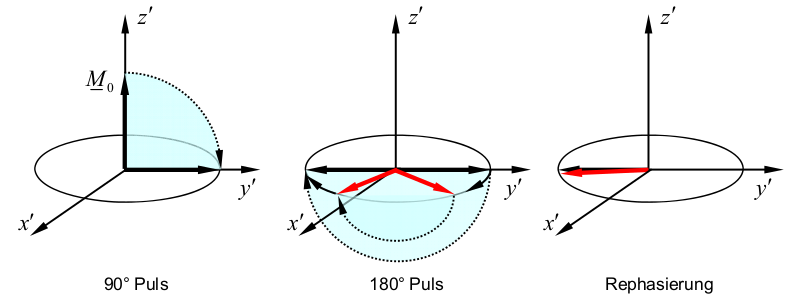
\includegraphics[width = .6\textwidth]{Spin-Echo.png}
  \caption{Rephasierung der Magnetisierung durch das Spin-Echo-Verfahren. Durch den \SI{90}{\degree}-Puls werden die Spins in die x'-y'-Ebene gekippt (dabei bezeichnet ' das drehende Koordinatensystem). Daraufhin dephasieren diese mit der Zeitkonstanten $T_2^*$. Der \textcolor{red}{rote} Pfeil symbolisiert dabei die schnelleren Spins. Durch den \SI{180}{\degree}-Puls werden alle Spins um die x'-Achse gekippt. Die schnelleren Spins holen die langsameren wieder ein und es kommt zur Rephasierung \cite{TOMO}.}
  \label{fig:Spin-Echo}
\end{figure}

Das dephasierende Signal wird dabei wieder rephasiert, indem ein \SI{180}{\degree}-Puls bei einer Zeit $\tau$ nach dem \SI{90}{\degree}-Puls geschaltet wird.
Durch den \SI{180}{\degree}-Puls werden die Spins um die x- oder y-Achse gedreht.
Weil diese aber ihre Präzessionsrichtung und Geschwindigkeit beibehalten, holen die schnellen Spins die langsameren wieder ein und es kommt zur Zeit $2\tau$ zur Rephasierung der Spins und damit zu einem messbaren Echosignal.
Die Einhüllende zwischen der Maximalamplitude nach dem \SI{90}{\degree}-Puls und dem Echosignal ist dabei durch Gleichung \eqref{eqn:T2Zeit} definiert.
Es können mehrere Spin-Echos hintereinander geschaltet werden, um innerhalb der $T_2$-Zeit viele Echosignale zu erzeugen.

Da der \SI{180}{\degree}-Puls nie exakt auf \SI{180}{\degree} geschaltet werden kann, gibt es kleine Abweichungen der Spinlage aus der x-y-Ebene, die mit jedem Spin-Echo zunimmt.
Im Signal erscheint dies als eine schnellere Dephasierung mit einer kleineren $T_2$-Zeit.
Um die Abweichung zu verhindern, wird der \SI{180}{\degree}-Puls um eine Phase von \SI{90}{\degree} zu dem \SI{90}{\degree}-Puls verschoben.
Die Phasenverschiebung bewirkt, dass die Spins nicht, wie z.B. beim \SI{90}{\degree}-Puls, um die x'-Achse (rotierendes Koordinatensystem), sondern um die y'-Achse gekippt werden.
Mit jedem zweiten \SI{180}{\degree}-Puls werden die Spins dann mit der selben Abweichung gekippt, wodurch sie wieder in der x-y-Ebene liegen.
Eine schematische Darstellung der Meiboom-Gill-Methode ist in Abbildung \ref{fig:Meiboom-Gill} dargestellt.

\begin{figure}[H]
  \centering
  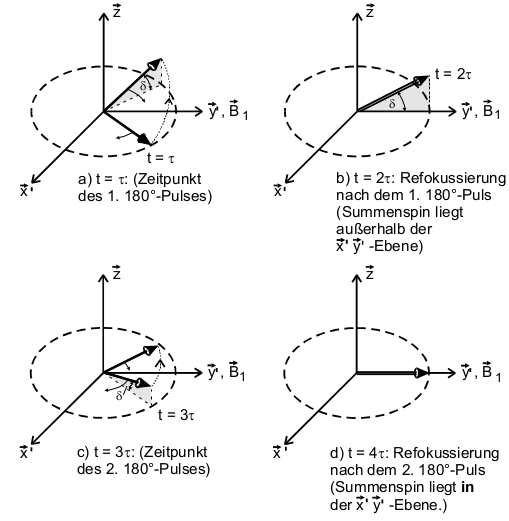
\includegraphics[width = .4\textwidth]{Meiboom-Gill.png}
  \caption{Darstellung der Meiboom-Gill-Methode. \textbf{a)} Durch eine Abweichung des \SI{180}{\degree}-Pulses werden die Spins um den Winkel $\delta$ aus der x-y-Ebene gekippt. \textbf{b)} Die Spins rephasieren außerhalb der x-y-Ebene. \textbf{c)} Durch den zweiten \SI{180}{\degree}-Puls werden die Spins nach "unten" gekippt, die Abweichung $\delta$ bleibt dabei gleich, wodurch die Spins wieder in der x-y-Ebene liegen und dort rephasieren \textbf{d)} \cite{Finke}.}
  \label{fig:Meiboom-Gill}
\end{figure}

%%%%%%%%%%%%%%%%%%%%%%%%%%%%%%%%    Diffusion    %%%%%%%%%%%%%%%%%%%%%%%%%%%%%%%%%%%%%%%%

\subsection{Diffusion}

Wird ein Gradienten in das statische $B_1$-Feld geschaltet, spüren die Spins lokal unterschiedliche Lamorfrequenzen.
Durch die Brownsche Molekularbewegung wechseln die Moleküle während der Zeit $2\tau$ nach dem \SI{90}{\degree}-Puls ihren Ort.
Die Rephasierung der Spins wird somit gestört und die Signalamplitude nimmt schneller ab, als in Gleichung \eqref{eqn:T2Zeit} beschrieben.
Für die Zeit $2\tau$, also dem Zeitpunkt des rephasierten Echos, beträgt die die Magnetisierung der Probe
\begin{equation}
  M(2\tau) = M_\text{x$_0$,y$_0$} \cdot e^{(\frac{-2\tau}{T_2})} \cdot e^{(\frac{-\tau^3}{T_\text{D}})} \, .
  \label{eqn:Diffusion}
\end{equation}
Der neue Exponentialtherm beschreibt dabei die Abnahme des Signals mit der Zeitkonstanten
\begin{equation}
  T_\text{D} = \frac{3}{2D \gamma^2 G^2}\,.
  \label{eqn:TDiffusion}
\end{equation}
Dabei ist $D$ der Diffusionskoeffizient und $G$ der Feldgradient im Probenkopf.

%%%%%%%%%%%%%%%%%%%%%%%%%%%%%%%%    Aufbau    %%%%%%%%%%%%%%%%%%%%%%%%%%%%%%%%%%%%%%%%

\section{Aufbau}
Dem Aufbau liegen zwei Permanentmagneten sowie die Sende- und Empfangsspule zugrunde.
Eine Zeichnung dieser ist in Abbildung \ref{fig:NMR-Magenten} gezeigt.
Durch die Permanentmagneten wird das statische Magnetfeld B$_0$ erzeugt, die Spule erzeugt die Radiofrequenzpulse für das B$_1$-Feld und ist direkt um den Probenkopf gewickelt.

\begin{figure}[H]
  \centering
  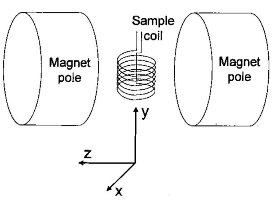
\includegraphics[width = .4\textwidth]{NMR-Magnete.png}
  \caption{Spulen zur Erzeugung der Magnetfelder. Die großen Permanentmagneten erzeugen das statische B$_0$-Feld. Die, senkrecht zu den Permanentmagneten um den Probenkopf gewickelte Spule erzeugt die B$_1$-Pulse und misst die Signale der Probe \cite{Aachen}. }
  \label{fig:NMR-Magneten}
\end{figure}

In Abbidung \ref{fig:Aufbau} ist der gesamte Aufbau schematisch dargestellt.
Herzstück des Aufbaus ist der Pulsgenerator.
An diesem können zwei unterschiedliche Pulse \textbf{A} und \textbf{B} eingestellt werden.
Puls \textbf{A} wird immer als Erstes vom Pulsgenerator erzeugt.
Die Pulslänge von \textbf{A} kann am Pulsgenerator eingestellt werden, genauso wie die des Puls \textbf{B} und dem zeitlichen Abstand zwischen \textbf{A} und \textbf{B}.
Weiterhin kann für \textbf{B} die Wiederholungszahl eingestellt werden.
Der Pulsgenerator wiederholt automatisch die Sequenzen mit einer einstellbaren Periodendauer.
Außerdem ist der Pulsgenerator mit dem Oszilloskop verbunden, um den Trigger des Oszilloskop auf einen der beiden Pulse zu setzen.

Der Frequenzgenerator wandelt die Pulse des Pulsgenerators in Radiofrequenzpulse um und gibt diese an die Spule weiter.
An ihm kann auch die Auswahl getroffen werden, ob der \SI{180}{\degree}-Puls um \SI{90}{\degree} zum \SI{90}{\degree}-Puls verschoben ist.

\begin{figure}[H]
  \centering
  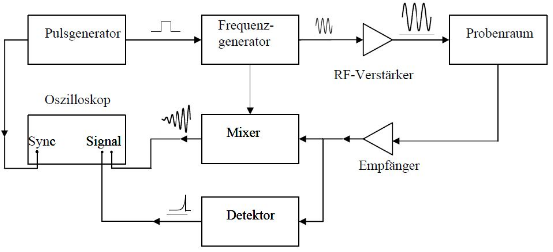
\includegraphics[width = .7\textwidth]{Aufbau.png}
  \caption{Aufbau der NMR-Versuchs \cite{Aachen}.}
  \label{fig:Aufbau}
\end{figure}



%%%%%%%%%%%%%%%%%%%%%%%%%%%%%%%%    Durchführung    %%%%%%%%%%%%%%%%%%%%%%%%%%%%%%%%%%%%%%%%

\section{Durchführung}
Der Versuch gliedert sich grob in zwei Abschnitte. Die Justage wird mit einem Gemisch aus Wasser und Kupfersulfat (\ce{CuSO_4}) und die Messungen der $T_1$-Zeit, $T_2$-Zeit und des Diffusionskoeffizienten an einer 1-Butanol Probe durchgeführt.

%%%%%%%%%%%%%%%%%%%%%%%%%%%%%%%%    Justage    %%%%%%%%%%%%%%%%%%%%%%%%%%%%%%%%%%%%%%%%

\subsection{Justage}
Zur Justage des Aufbaus wird die \ce{CuSO_4}-Probe in den Probenkopf gesteckt und die Startparameter aus Tabelle \ref{tab:Startparameter} eingestellt.
Die Frequenz wird so eingestellt, dass das Signal möglichst wenig Schwingungen aufweist und exponentiell gegen Null fällt.
Weiterhin wird die Phase so gewählt, dass möglichst das gesamte Signal in einem Kanal zu sehen ist.
Mit den Drehreglern werden die Gradienten (Shims) und somit die Feldhomogenität verändert. Die Einstellungen werden so gewählt, dass der FID nach einem Zeitraum von \SI{2}{\milli\second} noch mindestens ein Drittel seiner maximalen Intensität besitzt.
Die Pulslänge des \SI{90}{\degree}-Puls wird so eingestellt, dass die Amplitude des FID maximal ist. Für den \SI{180}{\degree}-Puls wird die doppelte Zeit des \SI{90}{\degree}-Puls gewählt.

\begin{table}[H]
  \centering
  \caption{Startparameter der Konsole. Zur Justage werden jediglich die Frequenz $F$ und die Phase $\phi$ verändert. Die Pulslänge $A$, die Anzahl der \textbf{B}-Pulse $N$, und die Periodendauer $P$ werden unverändert gelassen.}
  \label{tab:Startparameter}
  \begin{tabular}{ccc}
    \toprule
    Frequenz $F$ & \SI{21.7}{\mega\hertz} \\
    Pulslänge $A$ & \SI{2}{\micro\second} \\
    Anzahl \textbf{B}-Pulse $N$ & 0 \\
    Periode $P$ & \SI{0.5}{\second} \\
    Shims & $x = \num{1.0}, \,  y = \num{-5.0}, \, z = \num{3.7}, \, z^2 = \num{-2.4}$ \\
    \bottomrule
  \end{tabular}
\end{table}

%%%%%%%%%%%%%%%%%%%%%%%%%%%%%%%%    Durchführung T1 Butanol    %%%%%%%%%%%%%%%%%%%%%%%%%%%%%%%%%%%%%%%%

\subsection{$T_1$-Messung von 1-Butanol}
Zur Messung der $T_1$-Zeit wird die Inversion Recovery genutzt.
Dazu wird der erste Puls (\textbf{A}) als ein \SI{180}{\degree}-Puls und der zweite Puls (\textbf{B}) als \SI{90}{\degree} geschaltet.
Es wird nur ein \SI{90}{\degree}-Puls geschaltet.
Die Periode, also der Abstand zwischen zwei \SI{180}{\degree}-Pulsen wird zuerst auf $P=\SI{10}{\second}$ gestellt.
Der Pulsabstand \tau zwischen Puls \textbf{A} und Puls \textbf{B} wird dann in einem Bereich von $\tau \in [\SI{1}{\milli\second}, \SI{10}{\second}]$ weiter erhöht, bis die maximale Amplitude des FID auf der negativen Achse liegt.
Für jeden Pulsabstand wird die Amplitude des FID nach Puls \textbf{A} gemessen, dafür muss gegebenenfalls der Messbereich des Oszilloskops vergrößert werden, um das Signal nach Puls \textbf{A} zu detektieren.
Bei Werten von $\tau > \SI{1}{\second}$ wird die Periode auf $ P =\SI{10}{\second} + \tau$ erhöht.
Im Bereich des Nulldurchgangs werden mehr Messwerte als an den Rändern des Messbereichs bestimmt, um eine größere Genauigkeit für die Ausgleichsrechnung zur Bestimmung der $T_1$-Zeit zu erzielen.

%%%%%%%%%%%%%%%%%%%%%%%%%%%%%%%%    Durchführung T2   %%%%%%%%%%%%%%%%%%%%%%%%%%%%%%%%%%%%%%%%

\subsection{$T_2$-Messung von 1-Butanol}
Zur Messung der $T_2$-Zeit wird die Meiboom-Gill-Pulssequenz genutzt.
Die Pulslängen für \textbf{A} und \textbf{B} werden getauscht, sodass Puls \textbf{A} nun als \SI{90}{\degree} und Puls \textbf{B} als \SI{180}{\degree}-Puls geschaltet wird.
Die Anzahl der \textbf{B}-Pulse wird auf $N=100$ gestellt, die Periode wird auf das Dreifache der $T_1$-Zeit von 1-Butanol eingestellt.
In diesem Fall wird für die Periode $P = \SI{3.6}{\second}$ geschätzt.
Mit dem Schalter \textbf{MG} wird die Phase von Puls \textbf{B} um \SI{90}{\degree} zu Puls \textbf{A} verschoben.
Der Pulsabstand $tau$ wird so gewählt, dass die Echoamplitude nach dem letzten \textbf{B}-Puls in etwa \sfrac{1}{3} des ersten Echosignals entspricht.
Es wird mit dem Oszilloskop ein Bild einer Periode mit 100 Echosignalen aufgenommen und die Daten des Oszilloskops gespeichert.
Weiterhin wird ein Bild einer Messung ohne die Phasenverschiebung des \SI{180}{\degree}-Puls von \SI{90}{\degree} aufgenommen. Dazu wird der Schalter \textbf{MG} auf \textbf{off} gestellt.

%%%%%%%%%%%%%%%%%%%%%%%%%%%%%%%%    Diffusionsmessung    %%%%%%%%%%%%%%%%%%%%%%%%%%%%%%%%%%%%%%%%

\subsection{Diffusionsmessung}
Zur Auswahl einer möglichst kleinen Schichtdicke wird der z-Gradient auf den höchsten Wert gestellt und umgepolt.
Die weiteren Gradienten bleiben unverändert.
Puls \textbf{A} wird weiterhin als \SI{90}{\degree} und Puls \textbf{B} als \SI{180}{\degree} geschaltet.
Es wird pro Periode ein Puls \textbf{B} geschaltet.
Die Periode bleibt weiterhin bei $P = \SI{3.6}{\second}$.
Nun wird der Pulsabstand ab $\tau = \SI{100}{\micro\second}$ erhöht und jeweils die Maximalamplitude des Echosignals nach Puls \textbf{B} gemessen.
Der Pulsabstand wird so lange erhöht, bis das Echosignal nicht mehr vom Untergrundrauschen zu unterscheiden ist.
Für eine Messung mit einem kleinen Pulsabstand wird das gesamte Echosignal mit dem Oszilloskop aufgenommen und abgespeichert.
